\section{MongoDB and Big Data}
In terms of Mobile Applications, IoT, Industry 4.0 and cloud-computing, data is vast, unstructured, sometimes unwieldy and complicated. In this context, Big Data is identified by its velocity, variety and volume. Therefore, requirement and expectations has changed how to store, process and analyze data. It has led to the development of NoSQL databases such as MongoDB\cite{MongoDBInc.2013}.
\\
However, in the era of Big Data, there a 2 kind of database solutions for facing Big Data. We distinguish operational Big Data Systems and analytical Big Data solutions. Features of Operational Big Data Systems provides real-time, interactive, dynamic workloads that ingest and store data. MongoDB belongs to this category and is a popular technology for operational Big Data applications\cite{MongoDBInc.2013}.
\\
On the other hand, Analytical Big Data technologies are useful for retrospective, sophisticated analytics of your data. A most-known example of an Analytical Big Data technology is Apache Hadoop. Hadoop is designed for storing and processing large sets of data on a distributed environment based on commodity servers and storage. It is an open-source Apache project, which consists of a distributed file system called HDFS (Hadoop Distributed File System) and a data processing and execution model called MapReduce\cite{Wadkar2014}.
\\
Choosing between operational and analytical Big Data solution isn’t the right way of thinking about facing this Decision. Many organizations are harnessing the power of Hadoop and MongoDB together to create complete big data applications. At the one hand, MongoDB powers the online, real time operational application, serving business processes and end-users, exposing analytics models created by Hadoop to operational processes. At the other hand, Hadoop consumes data from MongoDB, blending it with data from other sources to generate sophisticated analytics and machine learning models. Results are loaded back to MongoDB to serve smarter and contextually-aware operational processes – i.e., delivering more relevant offers, faster identification of fraud, better prediction of failure rates from manufacturing processes\cite{MongoDBInc.2013}.
\\
In the following, you see a Figure which shows a Design pattern how to combine these two technologies to be ready for a Big Data environment:
\begin{figure}[H]
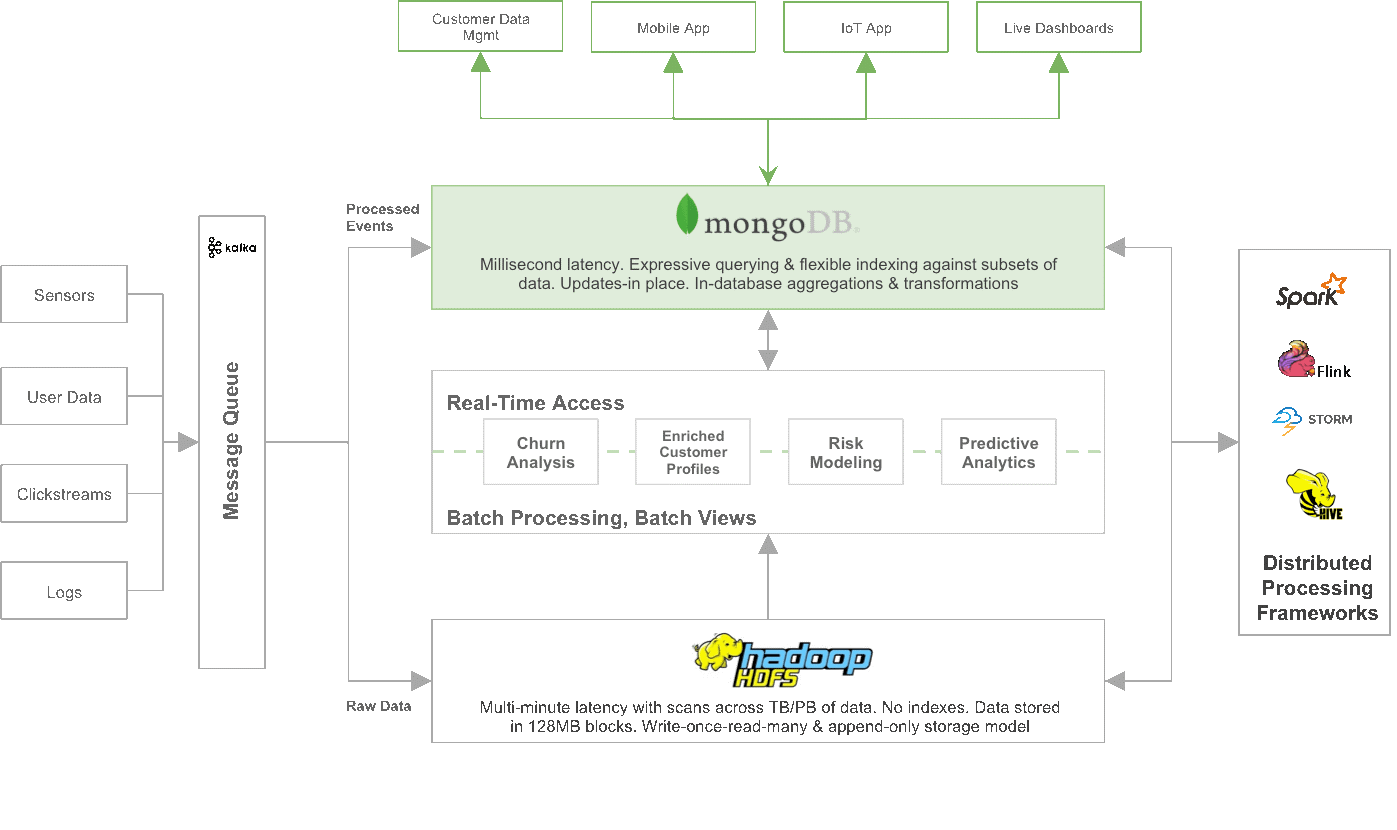
\includegraphics[width=\linewidth,keepaspectratio]{images/bigdata.png}
\caption{Design pattern for integrating MongoDB with Data Lake~\protect\cite{MongoDB2016}}
\end{figure}